% A simple Pentagon with TiKZ
% Author: Christoph Gerum <gerum@informatik.uni-tuebingen.de>

\documentclass{standalone}

\usepackage{tikz}


\begin{document}

%circle
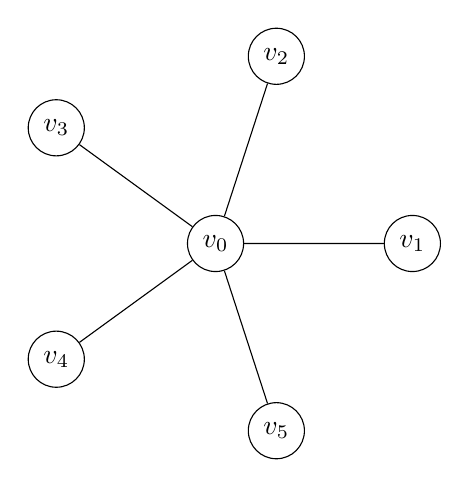
\begin{tikzpicture}[scale=2.5]
%  \draw [step=0.25cm,color=gray] (-1, -1) grid (1, 1);
  \tikzstyle {every node}=[draw,shape=circle];
  \path (0,0) node (v0) {$v_0$};
  \path (0*72:1cm) node (v1) {$v_1$};
  \path (1*72:1cm) node (v2) {$v_2$};
  \path (2*72:1cm) node (v3) {$v_3$};
  \path (3*72:1cm) node (v4) {$v_4$};
  \path (4*72:1cm) node (v5) {$v_5$};

  \draw (v0) -- (v1)
        (v0) -- (v2)
        (v0) -- (v3)
        (v0) -- (v4)
        (v0) -- (v5);
\end{tikzpicture}


\end{document}
